%+================+
%| DOCUMENT SETUP |
%+================+

% Set document class
\documentclass[xcolor=dvipsnames,11pt,paper=a4paper]{report}

% Include packages
\include{format/packages}
\include{format/python_code}
\addbibresource{bibliography/norms.bib}
%+----------------+
%| Document style |
%+----------------+

% Set default font to sans-serif
\renewcommand*{\familydefault}{\sfdefault}
% Make monospaced font a little smaller to fit text size
\let\tt\ttfamily
\renewcommand*{\ttfamily}{\small\tt}

% No horizontal paragraph indentation
\setlength{\parindent}{0pt}
\setlength{\parskip}{1em}

% Don't reset footnote counter with each chapter
\counterwithout{footnote}{chapter}

% Line spacing
\renewcommand{\baselinestretch}{1.5}

% Space before itemize/enumerate
\setlist[itemize]{topsep=-11pt}
\setlist[enumerate]{topsep=-11pt}

% Space after List of Figures etc.
\setlength\cftaftertoctitleskip{12pt}
\setlength\cftafterloftitleskip{12pt}
\setlength\cftafterlottitleskip{12pt}

% Set chapter style
\titleformat{\chapter}{\Huge\bfseries}{\thechapter. }{0pt}{\Huge\bfseries}
\titlespacing{\chapter}{0pt}{0pt}{20pt}
\titlespacing{\section}{0pt}{12pt}{0pt}
\titlespacing{\subsection}{0pt}{12pt}{0pt}
\titlespacing{\subsubsection}{0pt}{12pt}{0pt}

% Set author and title
\title{
	\Huge\textbf{Praxissemester bei Konzept Informationssysteme GmbH}\\\vspace{20pt}
	\includegraphics[width=0.3\textwidth]{graphics/konzept_logo.jpg}\break
	\huge{Bericht und Erfahrungen}
}
\author{
	\begin{tabular}{l l}
	Tom Georgi &
	\href{mailto:Tom.Georgi@htwg-konstanz.de}{\texttt{Tom.Georgi@htwg-konstanz.de}}\\
	&HTWG Konstanz\\
	&Angewandte Informatik, 4. Semester
	\end{tabular}
}
\date{01. September 2018 bis 28. Februar 2019}

%+================+
%| DOCUMENT START |
%+================+
\begin{document}
\pagenumbering{gobble} % No page numbers for the introduction!

%+------------+
%| Title page |
%+------------+
\begin{titlepage}
\begin{center}
\includegraphics[width=0.5\textwidth]{graphics/htwg.png}	
\end{center}
{\let\newpage\relax\maketitle}
\end{titlepage}


%+----------+
%| Abstract |
%+----------+
\begin{abstract}
In diesem Bericht geht es um mein Praktikum bei Konzept 
Informationssysteme GmbH,
welches ich im Rahmen meines Bachelorstudiums im Fach Angewandte 
Informatik im 4. Semester
absolviert habe.

Im Verlaufe dieses Berichts werde ich die mir zuteil gewordenen Aufgaben 
genauer beschreiben und erläutern. Dabei werde ich auf Herausforderungen 
und Probleme eingehen, sowie das Lösen und Überwinde dieser Hürden. 
Desweiteren werde ich meine Vorgehensweisen aufzeigen und erklären, sowie 
auf meine getroffenen Entscheidungen innerhalb des Projektes.


Meine Tätigkeit handelte von der Erstellung einer Testautomatisierungs 
Software im Bereich Avionik, die ein großes Spektrum im Bereich Embedded 
Systems umfasste. Dazu zählte das Ansteuern von mehreren 
unterschiedlichen Schnittstellen. Dabei war ich Teil eines neu 
angenommenen Kundeprojektes und bekam so ein umfassendes Bild der Arbeit 
innerhalb der Firma und durch Meetings auch direkt vor Ort beim Kunden.

Abschließend werde ich ein Fazit aus den gesammelten Erfahrungen ziehen.
Außerdem werde ich zusammenfassen, in welchen Aspekten mich das Praktikum 
weitergebracht hat.


%\pagebreak
\end{abstract}
%+-------------------+
%| Table of contents |
%+-------------------+
\tableofcontents
\pagebreak

%+----------------------+
%| List of Listings, 	|
%| List of Figures,  	|
%| List of Tables    	|
%| List of Norms	 	|
%| List of Bibliography |
%+----------------------+
\begingroup
\let\clearpage\relax
\lstlistoflistings
\listoffigures
\pagebreak
\printbibliography
\endgroup

%+---------+
%| Vorwort |
%+---------+
\pagenumbering{arabic} % turn page numbering on now
\setcounter{chapter}{-1} % Makes numbering start at 0, so ``real'' chapters start at 1.
\chapter{Vorwort}
\label{ch:0}

Zu Beginn möchte ich kurz etwas über die Firma erzählen und erläutern wie ich 
zu Konzept Informationssysteme gekommen bin.

Konzept Informationssysteme \footnote{\url{http://www.konzept-is.de/de}} ist ein Software- und Systemhaus für Industrieunternehmen mit den Schwerpunkten Softwareentwicklung, System Engineering und Qualitätssicherung im süddeutschen Raum, welches 20 Jahre Erfahrung in der Umsetzung von anspruchsvollen Projekten im IT-Umfeld hat. Dabei ist Konzept nicht nur auf eine Branche spezialisiert, sondern deckt ein Leistungspektrum von Analyse und Projektierung über Softwareentwicklung und Qualitätssicherung bis hin zu Beratung und Schulung ab.
Gegründet wurde die Firma 1994 und hat in diesem Zeitraum eine Größe von ca. 140 Mitarbeitern erreicht, welche sich auf die Standorte Meersburg, Ulm, München und Hünenberg(CH) aufteilt. 

Die Auftraggeber kommen aus den unterschiedlichsten Branchen wie zum Beispiel Avionik, Automotive, Raumfahrt, Energiesysteme, Produktion und Logistik sowie Verteidigungstechnik, Bahntechnik und Medizintechnik.

Im Verlaufe meines Studiums wurde mir immer klarer, dass Embedded Systems die Vertiefungsrichtung sein wird, welche ich nach meinem praktischen Studiensemester wählen würde. Durch einen Kommilitonen bin ich während der Connect Messe 2018 an der HTWG Konstanz \footnote{\url{https://www.htwg-konstanz.de}} auf Konzept aufmerksam geworden. Da mich der Bereich Avionik sehr interessiert, habe ich mich schließlich nach einem sehr informativen Gespräch dort beworben und schlussendlich ein halbes Jahr in dieser Firma verbracht. 

%+-----------+
%| Kapitel 1 |
%+-----------+
\chapter{Pin-Injection Automation für Diehl Aviation}
\label{ch:pia}

Das zu programmierende Projekt \ac{pia} wird für den Kunden Diehl Aviation
\footnote{\url{https://www.diehl.com/aviation/de/}} entwickelt, welches als semi-
automatisiertes Pin Injection Testing Programm fungieren soll.

Der Kunde Diehl muss die von ihnen entwickelten Geräte auf viele bestimmte Eigenschaften und
Ereignisse \ac{bzw} auch auf Gefahren testen, welche während eines Fluges auftreten können.
Einer dieser Tests ist der sogenannte Pin-Injection Test.
Bei diesem Test werden die Pins eines Fluggerätes auf Störungen und auch Beschädigungen im
Rahmen der Umweltqualitätsprüfung nach \cite{DO-160} getestet. Jeder Pin besitzt ein Interface
zum steuern von verschiedenen im Gerät verbauten Schaltern. Da jedes Interface andere
Eigenschaften besitzt, hat dementsprechend jedes dieser Interfaces unterschiedliche
Anforderungen (engl: "Requirements") die getestet werden müssen.
Demzufolge ist das Testen der Pins \ac{bzw} der Geräte sehr zeitaufwändig und kann im
Durchschnitt bis zu zwei Wochen dauern, je nachdem wie viele Pins das zu testende Gerät
besitzt.

\ac{pia} soll die Tests, welche normalerweise von einem Mitarbeiter von Hand abgearbeitet
werden, einlesen und nur durch eine vom Mitarbeiter angefertigte Konfigurationsdatei
automatisieren und verarbeiten.


\section{Projekteinarbeitung}
\label{sec:prj-einarbeitung}

Da das Projekt erst kurz vor meinem ersten Arbeitstag angenommen und mit Diehl beschlossen
wurde, stand bis auf die Aufgabenanforderung der Software noch nichts fest. Dementsprechend
konnte ich später in vielen Bereichen wie \ac{zb} die Programmiersprache oder auch die
Programmstruktur frei wählen und auch viele meiner Ideen mit ins Programm einfließen lassen.
Meine erste Aufgabe war es erst einmal das Verständnis für den eigentlichen Test zu bekommen,
welcher das Programm automatisieren soll, denn zu diesem Zeitpunkt war der vom Programm
ab zulaufende Testzyklus noch nicht vollständig festgelegt. 


\subsection{Aufgabe der zu programmierenden Software}
\label{subsec:aufgabe-software}

Die Aufgabe der zu entwickelten Software besteht darin, dass eine vom Mitarbeiter erstellte
Testkonfigurationsdatei, welche normalerweise von Hand abgearbeitet wird, eingelesen und
verarbeitet wird. Am Ende soll eine sogenannte Result Ouput Log File die Ausgaben der
Programmauswertung abspeichern und angeben ob ein Test gescheitert ist oder alles normal
verlief.
Bei der Verarbeitung eines Test Schritts wird ein Roboter angesteuert der maximal zwei
sogenannte Bananenstecker auf ein Board steckt, welches mit den Pins des zu testenden Gerätes
angeschlossen ist. Danach kann ein optionales \ac{micbac} Kommando an das am Pin anliegende
Interface geschickt werden, welches \ac{zb} einen internen Schalter umlegt. Danach wird ein
Puls mehrmals auf den Pin gefeuert. Dieser Puls hat eine vorgegebene Wellenform (engl:
"Waveform"), welche von einem angeschlossen Puls Generator generiert wird. Der Puls Generator
ist zugleich auch für die Anzahl der zu feuernden Pulse zuständig. Nach dem letzten
abgefeuerten Puls wird ein Bild vom Oszilloskop abgespeichert und mit einem vorher
aufgenommenen Referenzbild verglichen, um zu schauen ob der Pin \ac{bzw} sogar das komplette
Gerät beschädigt wurde oder ob alles in normal verlaufenden Bereich liegt. 


\subsection{Entwicklung der Programmstruktur}
\label{subsec:entw-prgstr}

Während meiner Praxisphase war die Entwicklung und im späteren Verlauf auch die
Weiterentwicklung der Programmstruktur ein großer Bestandteil meiner Arbeit. Da die Entwicklung
zum Teil etappenweise voran ging, mussten Teile der Programmstruktur relativ schnell und ohne
wirklich großen Aufwand modifizierbar, erweiterbar und zu einem gewissen Teil auch austauschbar
sein. 

\begin{figure}[H]
	\centering
	\includegraphics[width=0.75\textwidth, height=0.75\textwidth]{graphics/program_architecture.png}
	\caption{Programm Architektur}
	\label{fig:prg_architecture}
\end{figure}

Abbildung \ref{fig:prg_architecture} zeigt die entwickelte abstrakte Programmstruktur,
welche im Programm auch umgesetzt und benutzt wurde. Dort sieht man auch, dass das Programm
mehrere Interfaces für Oszilloskope und Puls-Generatoren ansteuert. Diese Anforderung wurde am
Ende so implementiert, dass sofern irgendeine neue Hardware Komponente eingebettet werden soll,
nur kleine Teile wie \ac{zb} die Auswahlmöglichkeit in der \ac{gui} erweitert werden muss. Die
eigentliche Programmstruktur wird dadurch nicht verändert, was die Flexibilität erhöht und es
so möglich ist das Programm nur durch hinzufügen einer neuen Datei, unter der Einhaltung von
einer bestimmten  Namensvergebung, zu erweitern. Erkennbar ist auch, dass die Aufgaben in
unterschiedliche Interfaces unterteilt wurden, was die Programmübersicht erhöht und  interne
Abhängigkeiten verringert. Dadurch sind \ac{zb} teile der \ac{gui} des öfteren ohne großen
aufwand schnell austauschbar gewesen, was mir im Verlaufe des Praktikums öfters mal sehr viel
Zeit eingespart hat.

	
\subsection{Python 3 als Programmiersprache}
\label{subsec:py3_as_lang}

Wie schon in Kapitel \ref{sec:prj-einarbeitung} erwähnt war es mir frei zu wählen, in welcher
Programmiersprache ich das Projekt realisieren möchte. Meine Entscheidung fiel dabei schnell
auf \cite{Python} 3, da auch die Erfahrung mit dieser Sprache auf der Seite des Kunden sehr 
groß war. Den Vorteil in dieser Sprache sehe ich darin, dass \cite{Python} eine sehr aktuelle 
und dynamische Programmiersprache ist, welche sich schnell weiterentwickelt. 

Das Hauptmerkmal von \cite{Python} ist die Lesbarkeit und wird durch Code Style Richtlinien und
Idiome realisiert. Diese Lesbarkeit wird auch \textit{Pythonic Way} genannt. Die Idiome in
\cite{Python} lassen zukünftige Leser genau verstehen, was der Code machen soll, während die
Code Style Richtlinien für einen einheitlichen Code sorgen.

Die Softwareanforderung wie \ac{zb} Datensätze aus einer \ac{csv} Datei auszulesen und zu 
verarbeiten konnte mit Hilfe der von \cite{Python} zur Verfügung gestellten \ac{api} sehr 
schnell realisiert werden. Des weiteren standen \cite{Python} Module für das Verarbeiten von 
\ac{micbac} Kommandos aus einem vorherigen Projekt bereits zur Verfügung.


\section{Die Erste Simulation}
\label{sec:first_simulation}

Die erste Aufgabe am Projekt war das erstellen einer Simulation. Die Simulation sollte am 
Anfang nur die Architektur implementieren und die Ausgabe für den Benutzer simulieren. Im 
Verlaufe des Praktikums wurden dann diese Ausgaben mit echten Werten verknüpft.

Um zu garantieren, dass die Softwarequalität bestehen bleibt, habe ich auf dem interen GitLab
\footnote{\url{https://about.gitlab.com/}} Server von Konzept einen sogenannten GitLab Runner
\footnote{\url{https://docs.gitlab.com/runner/}} erstellt. 


\subsection{Konfigurieren des GitLab Runner}
\label{subsec:gitlab_runner}

Um den Runner nicht jedes mal beim einchecken neu aufbauen zu müssen und die Daten immer mit 
den selben Eigenschaften eingecheckt werden, habe ich ein \cite{Docker} Image, ein Speicherabbild eines Containers, erstellt.

\cite{Docker} wird zur Isolierung von Anwendungen mit Containervirtualisierung genutzt. Diese 
Container gewährleisten die Trennung und Verwaltung der auf dem Rechner genutzten Ressourcen 
und vereinfacht die Bereitstellung von Anwendungen, weil sich die Container leicht als Dateien 
transportieren und installieren lassen.

\begin{figure}[H]
	\centering
	\includegraphics[width=1\textwidth, height=0.25\textwidth]{graphics/pipeline.png}
	\caption{Konfigurierte Pipeline}
	\label{fig:pipeline}
\end{figure}

In Abbildung \ref{fig:pipeline} stellt die Pipeline die Schritte dar, die durchlaufen werden.
Dazu gehört die Erstellung einer \ac{api} aus den Python Doc-Strings, die Code Kompilierung, das durchlaufen der Unit Tests und das durchlaufen von \cite{Pylint}. \cite{Pylint} ist ein statisches Codeanalyse Tool, das unter anderem den Code auf die Einhaltung der in \cite{PEP8} beschriebenen Regeln prüft.


\subsection{Einlesen von CSV-Dateien}
\label{subsec:read_csv}

\begin{python}
def read_data(self, path):
	with open(path, 'r', newline='\r\n') as data:
    	reader = csv.DictReader(self.__skip_comments(data), delimiter=';')
        test_data = []
        for row in reader:
	        test_data.append(row)

        return test_data
            
def __skip_comments(self, lines):
	for index, line in enumerate(lines):
    	line = re.sub(re.compile(r'\s*#.*$'), '', line).strip()
        if not set(line.rstrip('\r\n').split(';')).difference(self.ref_head):
        	self.first_line = index + 2
        if line.startswith(';'):
            continue
        if line:
            yield line
\end{python}


\subsection{Erstellung einer GUI}
\label{subsec:create_gui}


%+-----------+
%| Kapitel 2 |
%+-----------+
\chapter{Ansteuerung des Oszilloskop}
\label{ch:osci}

Im weiteren Verlauf meines Praktikums wurde mir irgendwann die Ansteuerung und die Implementierung eines Oszilloskopes zu Teil. 
Abbildung \ref{fig:lc334am} zeigt das Lecroy LC334AM 500Mhz Oszilloskop, welches über die \ac{gpib} Schnittstelle mit dem Computer kommunizieren kann. Der \ac{gpib} von \ac{ni}\footnote{\url{http://www.ni.com/de-de.html}} ist ein Industriestandard, welcher als \ac{ieee}\footnote{\url{https://www.ieee.org/}} veröffentlicht wurde.

\begin{figure}[H]
	\centering
	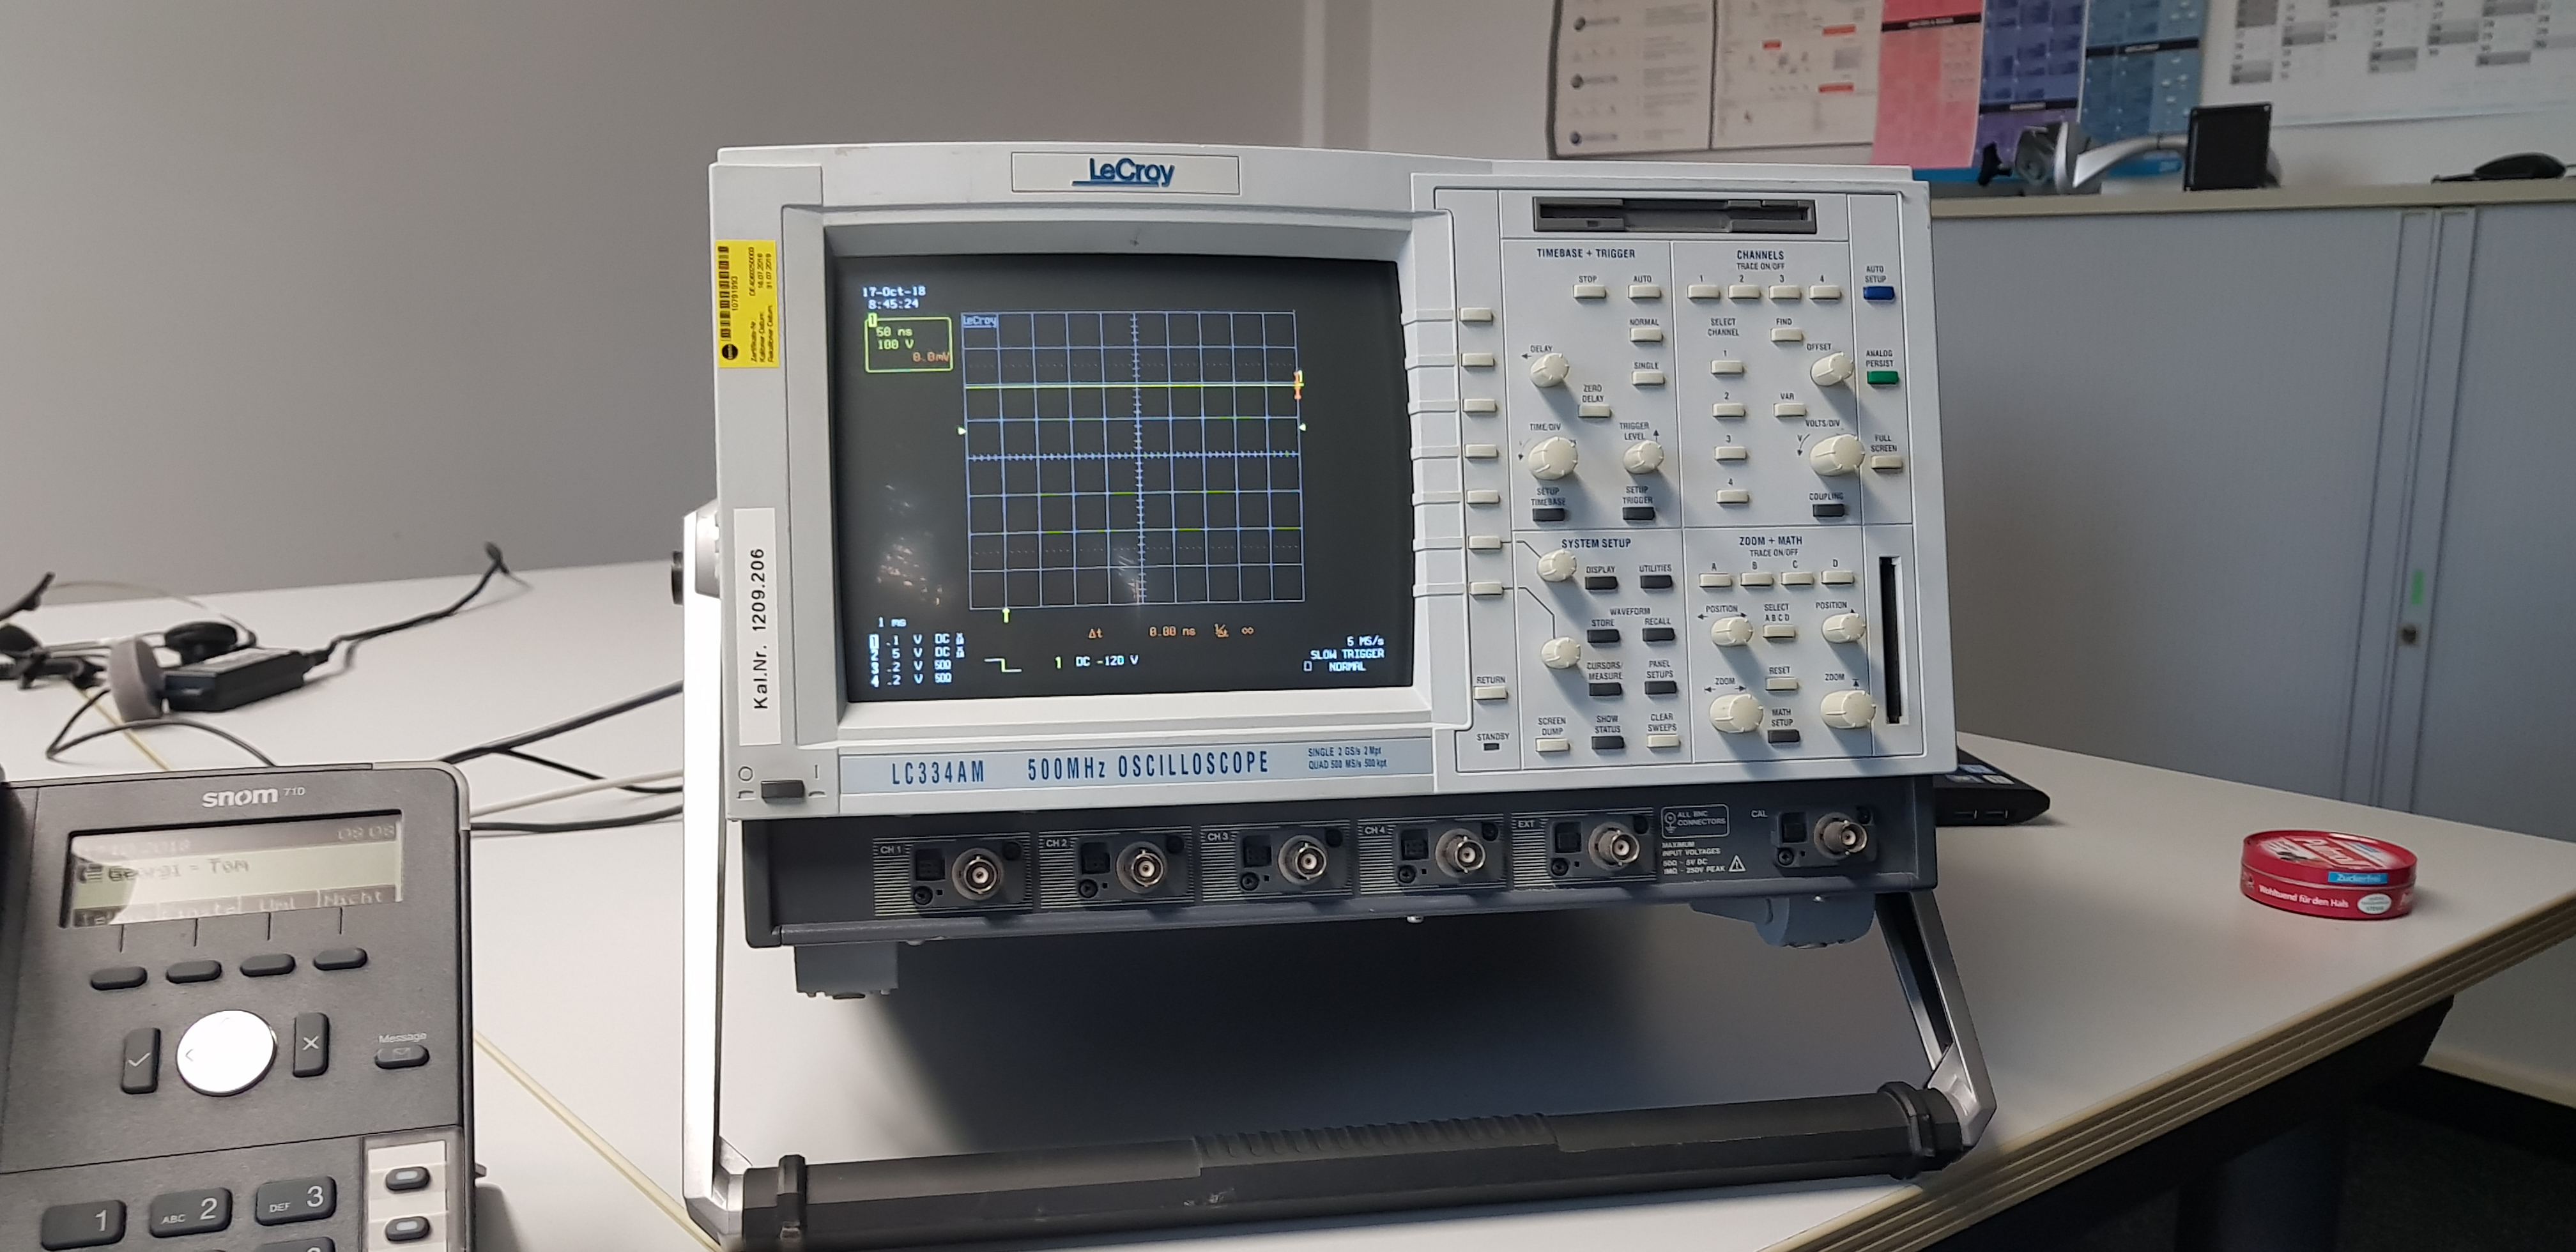
\includegraphics[width=1\textwidth, height=0.5\textwidth]{graphics/Programmed_Oscilloscope.jpg}
	\caption{Lecroy LC334AM 500MHz}
	\label{fig:lc334am}
\end{figure}




%+-----------+
%| Kapitel 3 |
%+-----------+
\chapter{Ansteuerung eines Remote Data Concentrator}
\label{ch:micbac}

Um das zu testende Pin-Interface anzusteuern und in die gewünschte Ausgangsposition zu 
bringen wird während dem \ac{pia}-Test bei manchen Test Situationen Befehle an die 
sogenannte \ac{uut} geschickt. Um dies in das Programm einbauen und testen zu können hat 
uns der Kunde Diehl einen \ac{rdc} zur Verfügung gestellt, der in Abb. 
\ref{fig:crdc-pins} und \ref{fig:crdc_top} zu betrachten ist.

\begin{figure}[H]
	\begin{minipage}{0.5\textwidth}
		\centering
		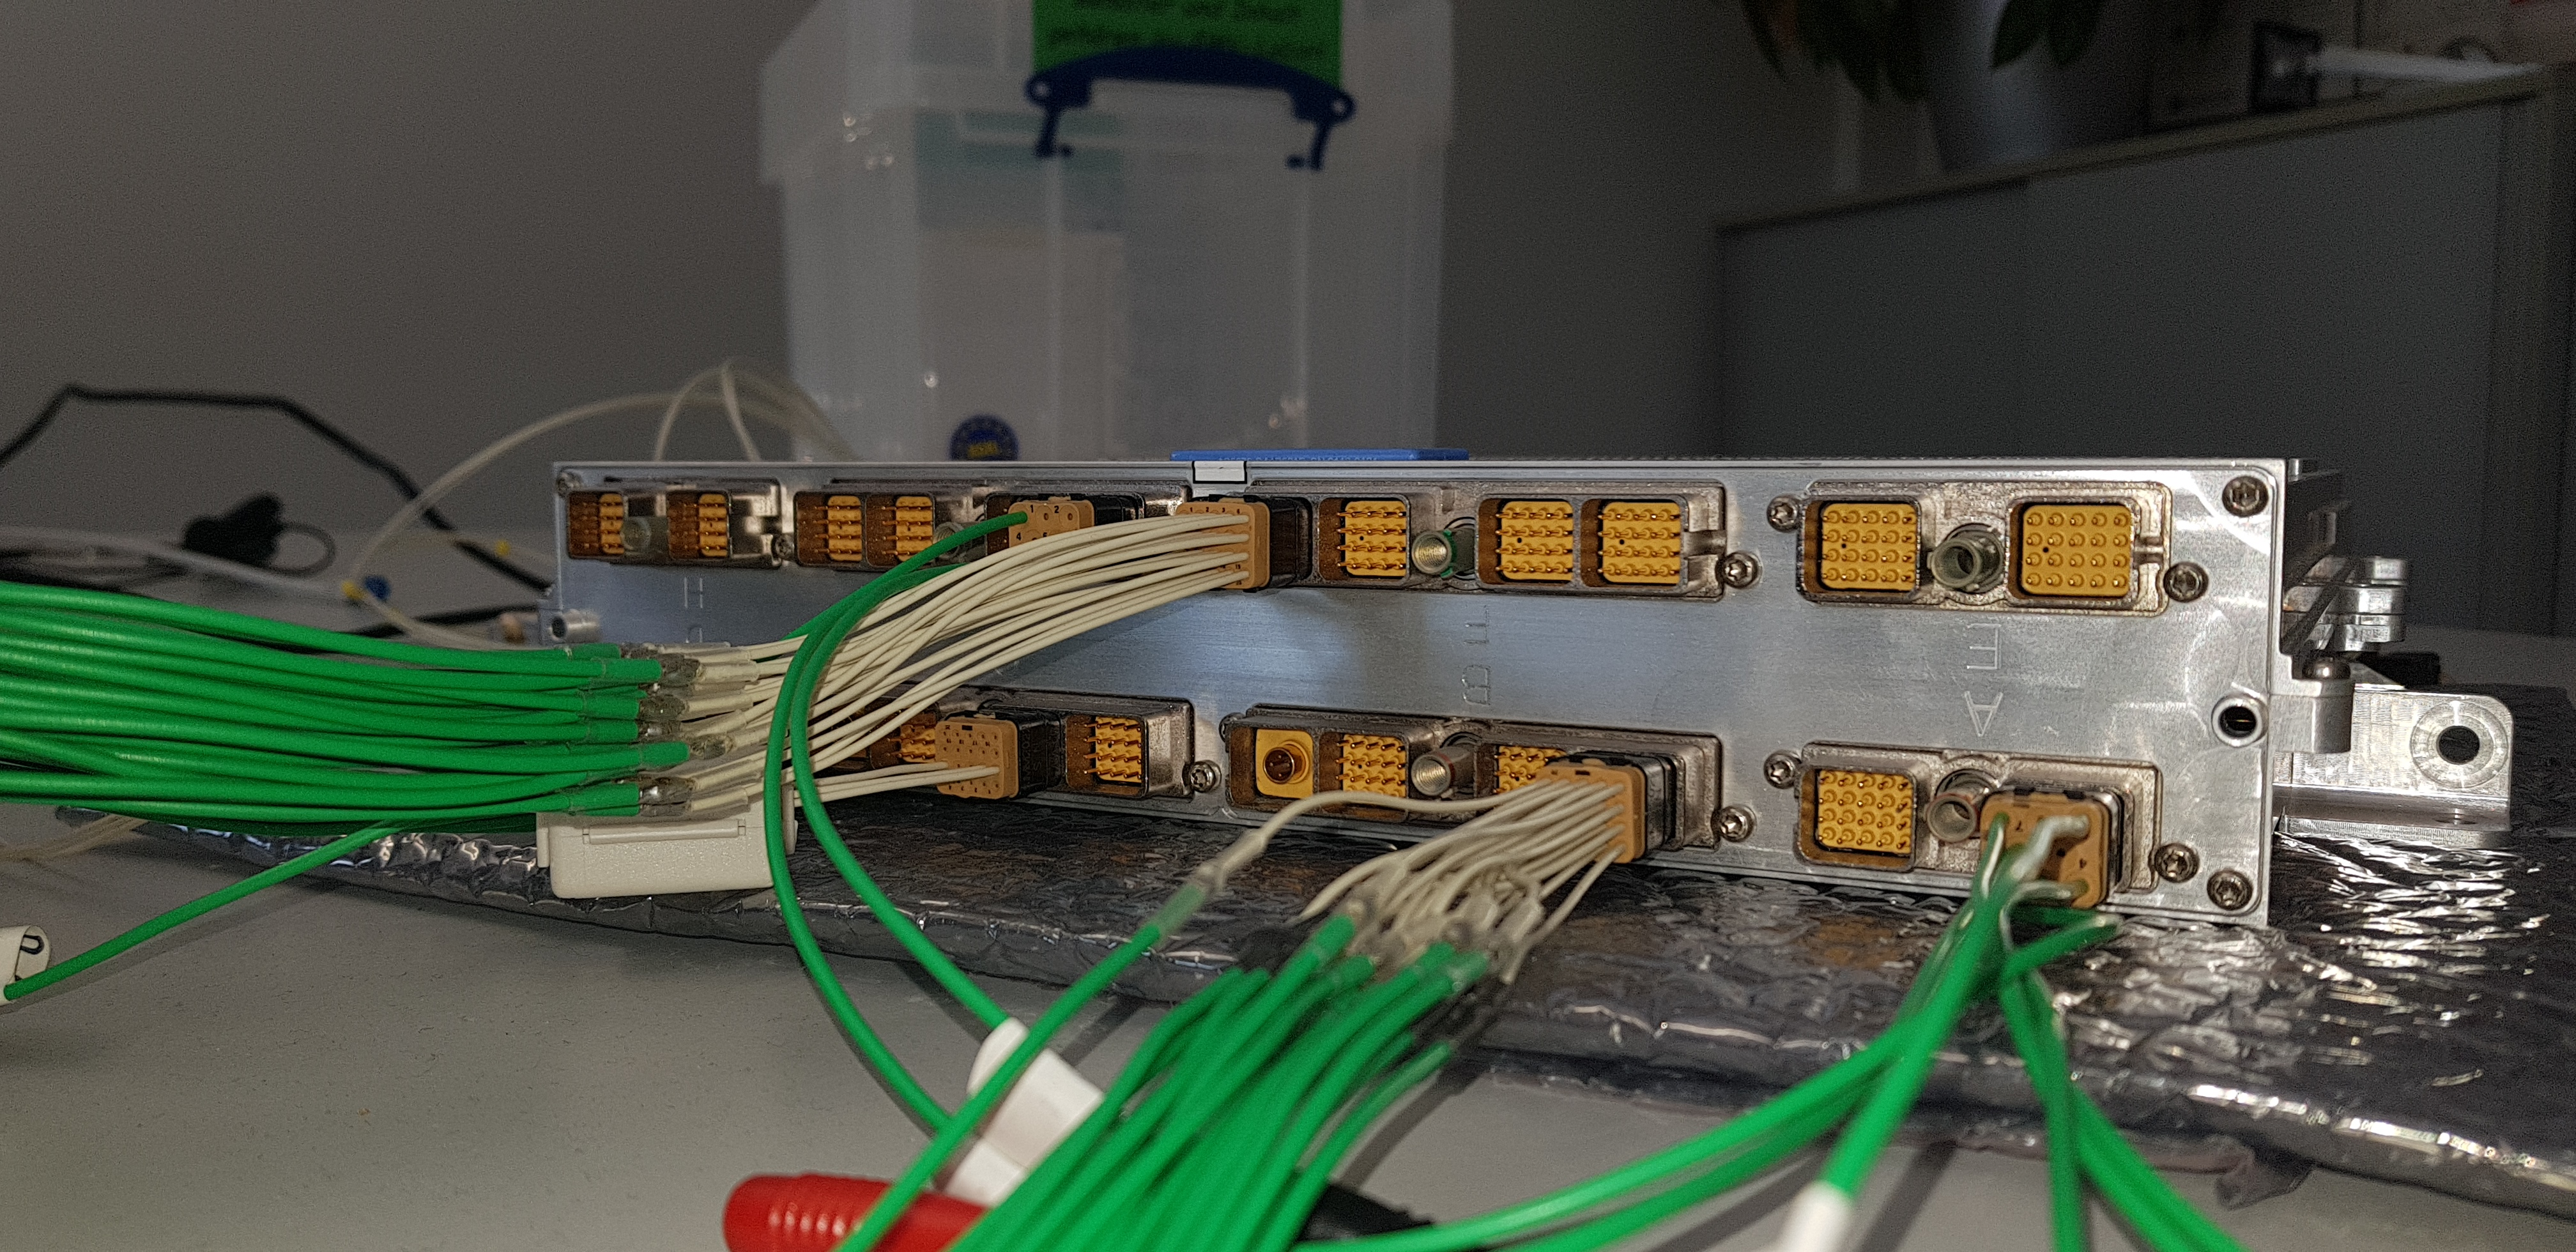
\includegraphics[width=\textwidth, height=0.5\textwidth]{graphics/crdc_1.png}
		\caption{RDC Type A Pins}
		\label{fig:crdc-pins}
	\end{minipage}
	\begin{minipage}{0.5\textwidth}
		\centering
		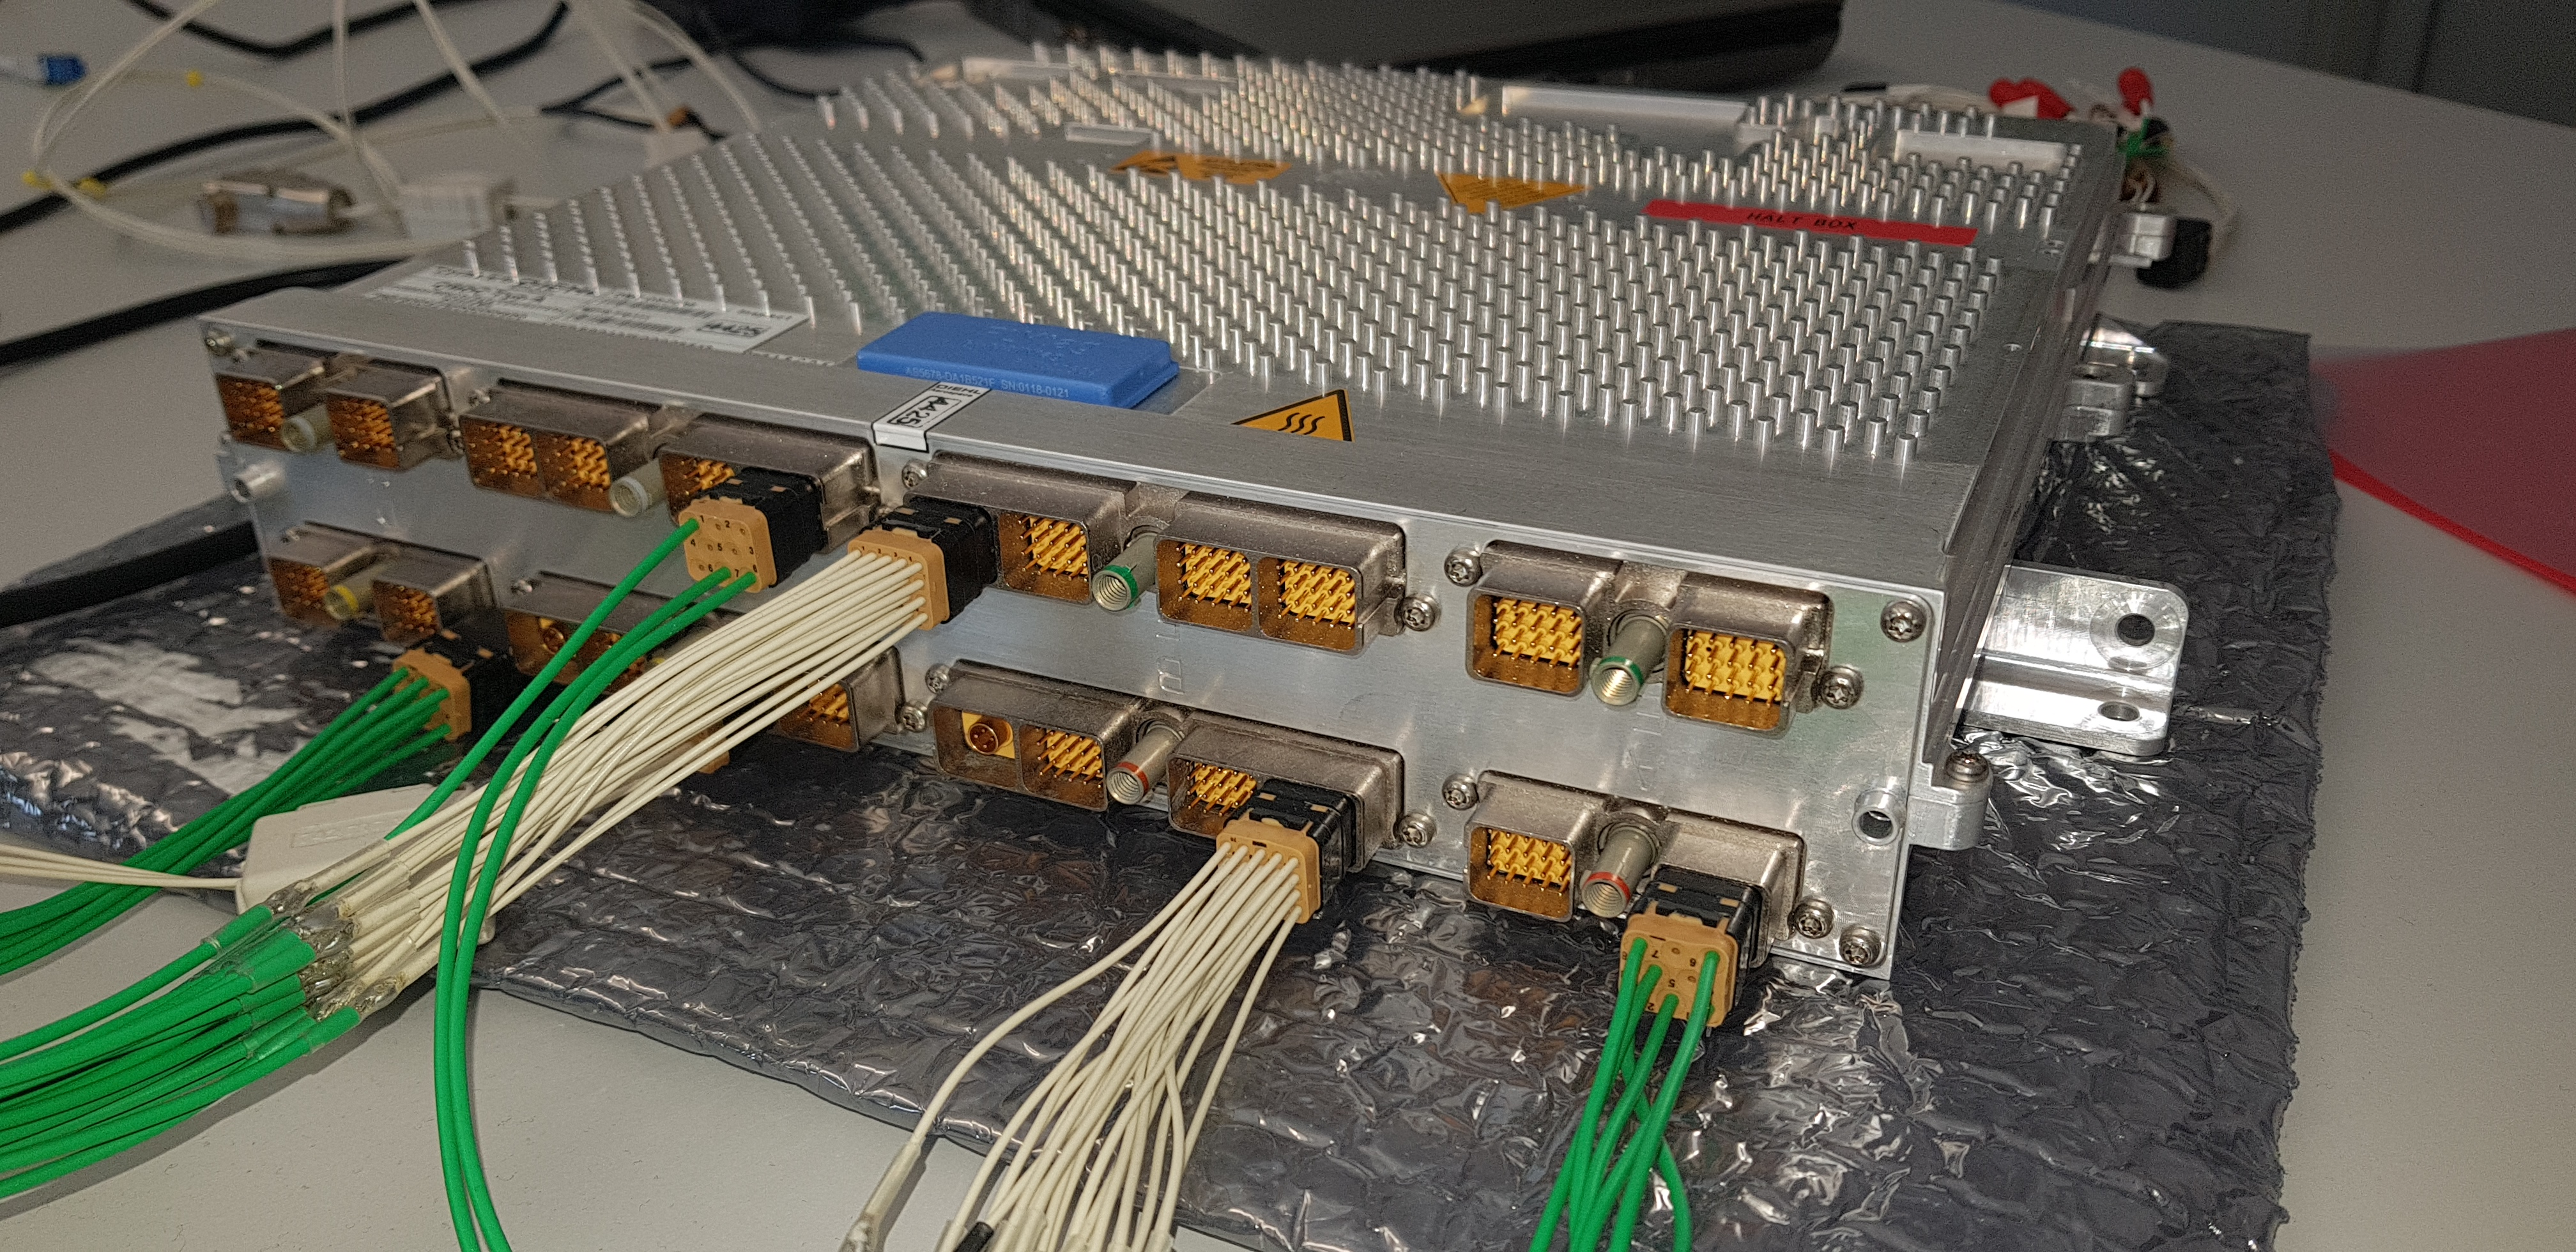
\includegraphics[width=\textwidth, height=0.5\textwidth]{graphics/crdc_2.png}
		\caption{RDC Type A}
		\label{fig:crdc_top}
	\end{minipage}
\end{figure}

Ein \ac{rdc} besteht aus einem Input/Output Interface um Verbindungen zu einem oder 
mehreren Input/Output Geräten und einem Netzwerk Interface, um eine Verbindung zu einem 
Fernprozessor zu ermöglichen.

%\section{Verbindung herstellen über das RS232-Interface}
%\label{sec:rs232-connection}

\section{Befehle Senden und Empfangen}
\label{sec:com-send-receive}

Um mit dem \ac{rdc} kommunizieren zu können werden Pins zu einem \ac{rs232}-Interface zur Verfügung gestellt. Mit Hilfe der Python-Bibliothek pySerial\footnote{\url{https://pyserial.readthedocs.io/en/latest/pyserial.html}} war es mir möglich ein Python Modul zu erstellen, dass sich um den Verbindungsaufbau, die Kommunikation und die Verbindungstrennung kümmert und kontrolliert. Mithilfe eines Threads konnte das Modul im Hintergrund auf den \ac{rs232}-Port hören ohne den Hauptteil des Programms dabei zu unterbrechen oder zu beeinträchtigen. Vorteil darin lag, dass der Workflow des Programms nur gestoppt wird wenn ein \ac{micbac}-Kommando an die \ac{uut} gesendet und eine Antwort erwartet wird. Dadurch war es mir möglich die Verbindung besser zu kontrollieren und Fehler wie \ac{zb} Datenverlust schneller zu erkennen. Des weiteren konnte ich so die Aufteilung der Programmstruktur besser einhalten und so einen besseren Überblick des Codes gewährleisten.

\subsection{Senden von MICBAC Commands}
\label{subsec:send-micbac}

Wie schon in Kapitel \ref{sec:com-send-receive} erwähnt werden zur Kommunikation sogenannte \ac{micbac}-Kommandos an die \ac{uut} geschickt. \ac{micbac}-Kommandos sind Befehle die über ein 32-Bit Mikrobussystem an die \ac{uut} gesendet werden und zur Steuerung und Abfrage von Information genutzt werden können. An jedem Pin eines \ac{rdc}s liegt ein anderes Interface an. Das bedeutet jedes Interface existiert in einem Gerät nur einmal. Nur der Typ des Interfaces kann gleich sein. Dadurch ist es möglich die Interface Typen in Python zu definieren und die Übersetzung der 32-Bit Befehle in die Typ-Definitionen zu implementieren.

\inputpython{scripts/send_micbac.py}{1}{15}{Send MICBAC Command}{lst:send-micbac}

Mithilfe von vorgefertigten Modulen von den Interface Typen aus einem anderen Projekt und den benötigten Adressinformationen, gespeichert in einer Tabelle, musste ich mich nur noch um das Einbinden der Module kümmern. Bevor ich die Module verwenden konnte musste der Code an manchen Stellen abgeändert und etwas um modelliert werden, da der Code in \citefield{Python}{note} 2 geschrieben wurde. In der eingelesen Testkonfiguration, die vom Tester erstellt wird, wird nur der Pin und der \ac{micbac}-Befehl angegeben was ein Problem darstellte, da der Pin nicht die benötigten Informationen enthielt. Durch  eingebettete Informationstabellen konnte ich in Hilfsmethoden dann die benötigten Informationen bestimmen, ein Objekt des benötigten Interface-Typen erstellen und den \ac{rs232}-Port registrieren. Am Ende musste ich nur noch den Befehl in der Interface-Typ-Instanz suchen und senden. Nachdem eine Antwort von der \ac{uut} empfangen wurde, wurden die Informationen an eine andere Methode übergeben und dort weiterverarbeitet.

\subsection{Empfangen von MICBAC Commands}
\label{subsec:receive-micbac}

\inputpython{scripts/receive_micbac.py}{1}{8}{Receive MICBAC Command}{lst:receive-micbac}

Nachdem Daten von der \ac{uut} empfangen wurde, werden diese an die Methode \textit{received\_msg()} übergeben. Da jeder Interface Typ unterschiedlich viele Datensätze als Antwort zurückschickt war es mir zum Ende hin nicht mehr möglich im Programm zu definieren wie viele Datensätze von einem Interface Typ benötigt werden um diese als eine vollständig gesendete Antwort zu bestimmen. Deshalb wurden erstmal alle Datensätze über einen vordefinierten Timer gesammelt und dann als Antwort in einer Liste gespeichert. Die Datensätze aus der Liste werden dann an die Methode \textit{start\_decode\_by\_msg()} übergeben. Dort werden sie in Adresse und Wert unterteilt und dann in der Interface-Typ-Instanz übersetzt und abgespeichert. Nach dem abspeicheren werden alle übersetzten Informationen aus der Interface-Typ-Instanz ausgelesen und zu einem lesbaren Text zusammengefügt. Der Text wird dann auf der \ac{gui} angezeigt und in einer Log-Datei abgespeichert.

%+-----------+
%|   Fazit   |
%+-----------+
\chapter{Fazit}
\label{ch:fazit}

Während meiner Tätigkeit bei Konzept Informationssysteme traf ich auf vielseitige Aufgaben, 
die oftmals mit vielen Problemen verknüpft waren. Durch das Anwenden von angeeigneten 
Kenntnissen im Rahmen meines Studiums, die Chance eigene Ideen mit einfließen zulassen und 
verschiedenste Herangehensweisen auszuprobieren verhalfen mir meist diese Probleme zu 
lösen. Manchmal stieß ich auf Herausforderungen wie \ac{zb} die Verarbeitung empfangener 
Daten vom LC334AM Oszilloskop, die ich nur durch alleiniges aneignen und verbinden von 
oftmals schwer zu findenden Informationen überwinden konnte.

Durch den Einstieg in ein komplett neu angenommenes Kundenprojekt hatte ich Einblick in 
viele Phasen der Umsetzung. Dazu zählte das Mitwirken bei Entwicklung und Gestaltung des 
Programmes, Wünsche und Anforderungen vom Kunden in Form von Meetings zu besprechen und ins 
Programm zu integrieren, sowie die Ausarbeitung von Lösungen verschiedenster auftretender 
Herausforderungen.

Mit diesen Einblicken konnte ich mich sowohl fachspezifisch, fächerübergreifend als auch 
persönlich weiterbilden und durch die vielen gesammelten Erfahrungen weiterentwickeln. 
Besonders mein Interesse im Bereich Embedded Systems hat sich nochmals gestärkt. Meine 
Fachkenntnisse, insbesondere Python, konnte ich in vielen Bereichen vertiefen. Weiterhin 
erlangte ich einen Blick auf den Firmenalltag, Abläufe und Veranstaltungen wie \ac{zb} das 
Präsentieren der Firma bei der Firmenmesse in der Hochschule Ravensburg-Weingarten
\footnote{\url{https://www.hs-weingarten.de/web/willkommen/startseite}} oder auch interne 
Veranstaltungen wie \ac{zb} den Jahresabschluss, der im Schloss Tettnang abgehalten wurde.

Die besonders freundlichen Kollegen sowie das mir zugeteilte Projekt selbst prägten mein 
Praktikum sehr positiv. Durch die Hilfe der Kollegen sowie das freundschaftliche 
miteinander sorgten dafür das es mir während der Arbeit an nichts mangelte. Gesten wie 
\ac{zb} das mitbringen von selbstgebackenen Kuchen von meinem Projektleiter erfreute meine 
Kollegen und mich jedes mal aufs neue. Abschließend kann ich ein Praxissemester bei Konzept 
absolut empfehlen.

%+----------------------+
%| Abkürzungsverzeichnis|
%+----------------------+
\section*{Abkürzungsverzeichnis}
\begin{acronym}[MICBAC]
\acro{bsp}[bsp.]{Beispiel}
\acro{bzw}[bzw.]{beziehungsweise}
\acro{gui}[GUI]{Graphical User Interface}
\acro{micbac}[MICBAC]{Micro System Bus Access Channel}
\acro{pia}[PiA]{Pin-Injection Automation}
\acro{zb}[z.B.]{zum Beispiel}
\end{acronym}


%+--------------------------+
%| Ehrenwörtliche Erklärung |
%+--------------------------+
\pagenumbering{gobble}
\chapter*{Ehrenwörtliche Erklärung}

Hiermit erkläre ich, dass ich diese Bachelorarbeit  selbstständig  und  nur  unter  Benutzung  
der  angegebenen  Literatur  und  Hilfsmittel  angefertigt  habe  und  alle  Ausführungen,  die  
wörtlich  oder  sinngemäß  übernommen  wurden,  als  solche  gekennzeichnet  sind.  Die  Arbeit  
hat  in  gleicher  oder  ähnlicher  Form  noch  keiner  Prüfungsbehörde  vorgelegen  und  ist  
auch  noch  nicht veröffentlicht. Ich bin mir bewusst, dass eine falsche Erklärung rechtliche 
Folgen haben wird.

\vspace{5cm}

\rule{3.5cm}{1pt} \hspace{1.5cm} \rule{10cm}{1pt}\\
Datum \hspace{4cm} Unterschrift\\



%+==============+
%| DOCUMENT END |
%+==============+
\end{document}

